\section{Flask Overview}
Flask adalah sebuah Micro Web Framework untuk Bahasa pemrograman Python, yang mana  mempermudah
seorang developer dalam membuat sebuah Aplikasi Website. Flask adalah Framework umum
yang bisa di aplikasikan untuk Project yang skalanya berbeda-beda. untuk sebuah 
instansi, hal itu dapat digunakan untuk aplikasi web yang kecil dalam cakupan jaringannya.
prinsip fundamentalnya sama, yang mana bisa dengan mudah dibuatkan projectnya dalam skala aplikasi
website seperti apa saja \cite{alemu2014rest}.

\section{Flask}
pada web server menyediakan sebuah flask yang dimaksud oleh flask yaitu digunakan hanya untuk suatu pengembangan dan pengujian. 
dan web server kini juga pengembangan flask sudah  dapat dijalankan secara terprogram dengan menerapkan metode app.run \(\). 
versi command yang  berfungsi lebih lama dan tidak pula memiliki perintah flask requidred serveryang untuk memulai dengan menjalankan 
skrip pada utama aplikasi.

\subsection{Methods dalam Flask}
Ada beberapa method dalam flask yang terdiri dari GET, PUT,POST dan DELETE seperti pada table dibawah \ref{methods}. 
Dari methods-methods tersebut masing-masing fungsinya berbeda, terutama untuk PUT akan dijelaskan lebih detail. 
PUT adalah metode yang digunakan untuk memperbarui sumber daya dengan konten yang diunggah. 
Method ini sangat fleksibel karena bisa berinteraksi dengan beberapa bahasa pemrograman lainnya seperti bahasa pemrograman pyhton.

\begin{table}[h]
    \caption{Methods Flask}
    \centering
    \begin{tabular}{cccc}
    \hline
    POST&GET&PUT&DELETE\\
    \hline
    \label{methods}
    \end{tabular}
\end{table}


\section{Flask dan Framework}
HTTP mendefinisikan seperangkat metode permintaan untuk menunjukkan tindakan yang diinginkan yang akan dilakukan untuk sumber daya tertentu. 
Meskipun mereka juga bisa menjadi kata benda, metode permintaan ini kadang-kadang disebut sebagai verba HTTP. 
Masing-masing menerapkan semantik yang berbeda, namun beberapa fitur umum digunakan bersama oleh mereka: mis. 
Metode permintaan dapat berupa safe, idempotent, atau cacheable.

\subsection{Perbandingan Framework Flask dan lain}
Ada beberapa framework yang menggunakan bahasa pemrograman pyton sebagai basisnya. Diantara lain, Django, Pyramid, Tornado, Bottle, Diesel , Pecan, Falcon dan sebagainya.
Pada pembahasan ini tentang penggunaan Flask sebagai Framework untuk menunjang cloud server yang dibuat. 
Flask adalah microframework berbasis python. Framework Flask dan Django bila dilihat dari segi proses, Flask lebih unggul dari Django. 
Flask jauh lebih ringan dan cepat dari pada Django dikarenakan Flask dibuat dengan ide menyederhanakan inti frameworknya seminimal mungkin. 
Flask dapat membantu kita membuat situs dengan sangat cepat dan efisien meskipun dengan library yang sederhana.

\subsection{Fitur Flask}
Ada beberapa fitur dalam flask yaitu adalah berisi 
\begin{enumerate}
    \item pengembangan server, 
    \item terdapat dukungan terintegrasi untuk pengujian unit, 
    \item RESTful request dispatching, 
    \item Menggunakan temple engine, 
    \item dukungan untuk secure cookies atau sisi klien sesi, 
    \item terdapat seratus persen WSGI 1.0 compliant, 
    \item berbasis Unicode, 
    \item dokumentasi yang ekstensif, 
    \item kompatibilitas Google App Engine dan terakhir Ekstensi yang tersedia untuk meningkatkan fitur-fitur yang diinginkan.
\end{enumerate}

\subsection{Method Flask PUT}
Web Service dapat didefenisikan sebagai sistem yang dirancang untuk mendukung interaksi antara berbagai macam mesin-mesin pada suatu jaringan.Web service menyediakan beberapa methode yaitu contohnya pada  HTTP untuk melakukan aktivitas HTTP tentu saja menggunakan perintahnya yaitu seperti  GET, POST, PUT atau DELETE dan fungsi dari perintah methode PUT yaitu untuk mengupdate atau memperbarui sebuah data.
fungsi dari flask PUT sendiri bukan hanya mengganti data saja tapi
juga digunakan sebagai perintah yang melakukan
penggantian semua data yang ada dengan data yang di update, sehingga
data yang tersedia dalam keadaan baru dan tidak terjadi error.
Source CODE untuk perintah flask PUT ini sendiri terdapat pada gambar \ref{4PUT} 
itu adalah contoh method flask PUT pada Python.

\subsubsection{PUT}
Put adalah metode yang digunakan untuk memperbaharui sumber daya. Ini melakukan operasi pembaruan. 
Tidak seperti POST, hanya mengeksekusi untuk memperbaharui sumber daya. Dalam PUT kita sama saja dengan kita 
melakukan aktivitas update, yang berarti dimana ada file yang sudah dibuat atau sudah jadi akan kita perbahurui 
dengan file yang baru dengan menggunakan perintah PUT.

\begin{figure}[ht]
    \centerline{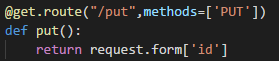
\includegraphics[width=1\textwidth]{figures/3put.PNG}}
    \caption{Contoh Flask PUT method}
    \label{4PUT}
\end{figure}

\subsection{Perbedaan POST dan PUT}
POST dan PUT tentunya memiliki perbedaan secara arti maupun kegunaanya. POST yang berarti methode yang digunakan untuk pembuatan
instance baru dari sumber daya yang berarti merupakan operasi untuk membuat bukan memperbaharui data yang sudah ada. 
Sedangkan PUT merupakan methode yang digunakan untuk memberbaharui data yang sudah ada. Jadi POST itu untuk membuat 
sedangkan PUT untuk memperbaharui.

\subsection{Cara Kerja Flask}
bagaimana itu bekerja
 di sini adalah fitur umum dari data permintaan. Untuk memberikan contoh, setiap deskripsi menyertakan nilai contoh untuk permintaan yang menekan / string /? Foo = bar & foo = baz dari browser kami.    

 \begin{itemize}
    \item endpoint: Ini reatures dari objek permintaan menentukan nama endpoint permintaan diarahkan, misalnya, return_string.    
    \item metode: Fitur ini dari objek permintaan menentukan metode HTTP dari permintaan saat ini, misalnya, GET.   
    \item view_args: fitur objek permintaan ini menentukan dict of view argumen fungsi yang diurai dari aturan rote URL misalnya 
\end{itemize}

\section{Struktur aplikasi Dasar}
Struktur Aplikasi Dasar 
Dalam bab ini, Anda akan belajar tentang berbagai bagian aplikasi labu. Anda juga akan menulis dan menjalankan aplikasi web flask pertama Anda. 
Inisialisasi 
Semua aplikasi Flask harus membuat instance aplikasi. Server web melewati semua permintaan yang diterimanya dari klien ke objek ini untuk ditangani, menggunakan protokol yang disebut antarmuka gerbang server web (WSGI, prononced "wiz-ghee"). 
Contoh aplikasi adalah objek dari kelas Flask, biasanya dibuat sebagai berikut: 

\begin{verbatim}
    from flask import Flask, request
    get = Flask(__name__)
    
    @get.route("/hello")
    def hello():
        return "Hello World"
\end{verbatim}


\section{Instalisasi Framework Flask}
syarat untuk melakukan instalisasi ini pastikan PC kalian sudah terinstal bahasa pemrograman Python dan virtualenv, setelah
itu lakukan cara seperti dibawah ini :
\begin{itemize}
    \item sudo pip install virtualenv 
    \item mkdir myproject (untuk membuat folder projectnya)
    \item cd myproject (untuk menuju ke direktori)
    \item virtualenv venv (instalisasi virtualenv)
    \item . venv/bin/activate (mengaktifkan virtualenv)
    \item pip install Flask (menambahkan library Flask menggunakan pip)
\end{itemize}
Dalam melakukan penginstalan tersebut ada yang dinamakan dengan Virtualenv, apa itu Virtualenv ?, Virtualenv merupakan alat yang
digunakan untuk membuat pengembangan di dalam lingkungan Python yang telah terisolasi dan kita bisa mengerjakan semua dalam
proses pengembagan yang akan kita perlukan. Jadi dengan adanya Virtualenv ini kita dapat mengembangkan project yang kita buat
dengan menggunakan bahasa pemrogramman Python.
Sebelum menggunakan Virtualenv, tentunya kita harus melakukan instalasi terlebih dahulu.
Virtualenv dapat diinstall dengan cara apt.
\begin{itemize}
	\item apt install virtualenv / apt install python-virtualenv
atau untuk python3,
	\item apt install python3-virtualenv
atau bisa juga menggunakan pip
	\item [sudo] pip install virtualenv
\begin{itemize}
kalian bisa menginstall menggunakan cara yang kalian sukai. Dalam penggunaan perintah [sudo], maka virtualenv akan menginstall
secara global.

\section{Konteks Aplikasi dan Permintaan}
Ketika Flask menerima permintaan dari klien, Flask harus membuat beberapa objek tersedia untuk fungsi tampilan yang akan menanganinya. Contoh yang baik adalah objek permintaan, yang merangkum permintaan HTTP yang dikirim oleh klien. Cara yang jelas di mana Flask bisa memberikan pandangan akses fungsi ke objek permintaan adalah dengan mengirimkannya sebagai argumen, tapi itu akan memerlukan evert fungsi tampilan tunggal dalam aplikasi untuk memiliki argumen estra.
jika tidak terjadi error maka dalam instalisasi kali telah berhasil

\section{flask methode}
Salah satu flask methode yaitu metode flaske methode yang digunakan pada saat Studies on O/W partition coefficient and absorption kinetics of geniposide in fructus gardeniae extract in rat intestine. Untuk menentukan koefisien partisi O/W tesebut geniopside dalam ekstara fructus gradien dan menyelidiki kinetik obsropsi yaitu menggukana methode sahke untuk menentukan koefisien O/W.

\section{Tanggapan megenai Flask}
Ketika Flask Memanggil fungsi tampilan, itu mengharapkan nilai kembalinya ke respon br untuk permintaan tersebut. Dalam banyak kasus, responsnya adalah string sederhana yang dikirim kembali ke klien sebagai halaman HTML. Tetapi protokol HTTP membutuhkan lebih dari string sebagai tanggapan atas permintaan. Bagian yang sangat penting dari respons HTTP adalah kode status, yang secara default ditetapkan oleh Flask menjadi 200, kode yang menunjukkan bahwa permintaan dilakukan dengan sukses.

\section{Flask Mode}
Mode framework flask adalah mode debug, dalam mode ini aplikasi bisa lebih opsional dieksekusi dalam mode debug. Dua modul pengembangan server yang sangat mudah disebut reloader dan debugger diaktifkan secara default.
Ketika reloader diaktifkan, flask menyimpan semua file kode sumber projek anda dan secara otomatis me-restart server ketika salah satu file diubah. 
Memilki server yang berjalan dengan reloader diaktifkan sangat berguna selama pengembangan, karena setiap kali anda memodifikasi dan menyimpan file sumber, server secara otomatis memulai ulang dan mengambil perubahan.

\section{Database di Flask}
Pada pembahasan ini kita akan menggunakan ekstensi yang salah satunya yaitu Flask-SQLAlchemy, ekstensi flask untuk menggunakn paket SQLAlchemy yang sudah dipackage sedemikian rupa sehingga lebih soft terhadap kode flask.
SQLAlchemy adalah sebuah Object Relational Mapper atau dengan singkatan ORM. ORM memungkinkan aplikasi untuk menggunakan database dengan data high level seperti kelas, objek, method dari pada menggunakan tabel dan kode SQL secara langsung. 
Tugas ORM adalah mentranslate operasi high level menjadi perintah database.

\section{Flask Security Architecture}
Arsitektur keamanan flask yaitu salah satu dari penggunaan teknologi yang ada. Yang dimaksud dengan arsitektur keamanan flask yaitu dapat digunakan untuk meyediakan suatu RAdAC yang menggambarkan bagimana dilakukannya dalam sebuah prototipe sistem di RAdAC. Yang dimaksud dari RAdAC adalah teknologi baru yang begitu penting dan sudah banyak mendapatkan perhatian dari banyak karena sebagai cara untuk mengubah kebijakan informasi pada saat ini.

\subsection{Database di Flask}
Pada pembahasan ini kita akan menggunakan ekstensi yang salah satunya yaitu Flask-SQLAlchemy, ekstensi flask untuk menggunakn paket SQLAlchemy yang sudah dipackage sedemikian rupa sehingga lebih soft terhadap kode flask. 
SQLAlchemy adalah sebuah Object Relational Mapper atau dengan singkatan ORM. ORM memungkinkan aplikasi untuk menggunakan database dengan data high level seperti kelas, objek, method dari pada menggunakan tabel dan kode SQL secara langsung. 
Tugas ORM adalah mentranslate operasi high level menjadi perintah database.

\subsection{Ikthisar Flask API}
Flask API adalah pengganti drop-in untuk Flask yang menyediakan implementasi API yang dapat dijelajahi mirip dengan apa yang disediakan oleh kerangka kerja REST Django. Ini memberi Anda konten yang dirundingkan dengan benar dan respons parsing permintaan cerdas:
Ambil, perbarui atau hapus instance catatan :

Dapatkan 
\begin{verbatim}
/ 1 /
HTTP 200 OK
content-Type: aplikasi / json
{
     "url": "http: //127.0.01: 5000/1 /".
     "text": "membangun kodez"
}
\end{verbatim}



